\documentclass[12pt,a4paper]{article}
\usepackage{graphicx}
\usepackage{gensymb}
\usepackage{amsmath}
\usepackage{amssymb}
\usepackage{bm}
\usepackage{tikz}
\usepackage{titlesec}
\usepackage{float}
\usepackage{mathtools}
\usepackage{caption}
\usepackage{subcaption}
\usepackage{minted}
\setminted{frame=single,framesep=10pt,breaklines,linenos}
\setcounter{secnumdepth}{4}
\tikzset{
    node distance=2cm, % specifies the minimum distance between two nodes. Change if necessary.
    }
\title{Case Study Modelling an Electronic Component}
\author{
  Azure Hutchings
  \and
  Jean-Luc Danoy
  \and
  Faris Saad S Alsubaie
}
\date{28 October 2019}
 
\begin{document}
 
\begin{titlepage}
\maketitle
\end{titlepage}

\renewcommand{\abstractname}{Executive Summary}
\begin{abstract}
Write Abstract Here
\end{abstract}

\pagebreak

\tableofcontents

\pagebreak

\section{Introduction}

\subsection{Purpose of the Report}
The following report investigates the steady-state heat distribution in a newly designed component. 
\\\\
The report will discuss how to numerically solve for the steady-state heat distribution, the efficient of different methods and the effect of different ambient temperatures.

\subsection{The Maths of the Problem}

\begin{figure}[H]
	\center
	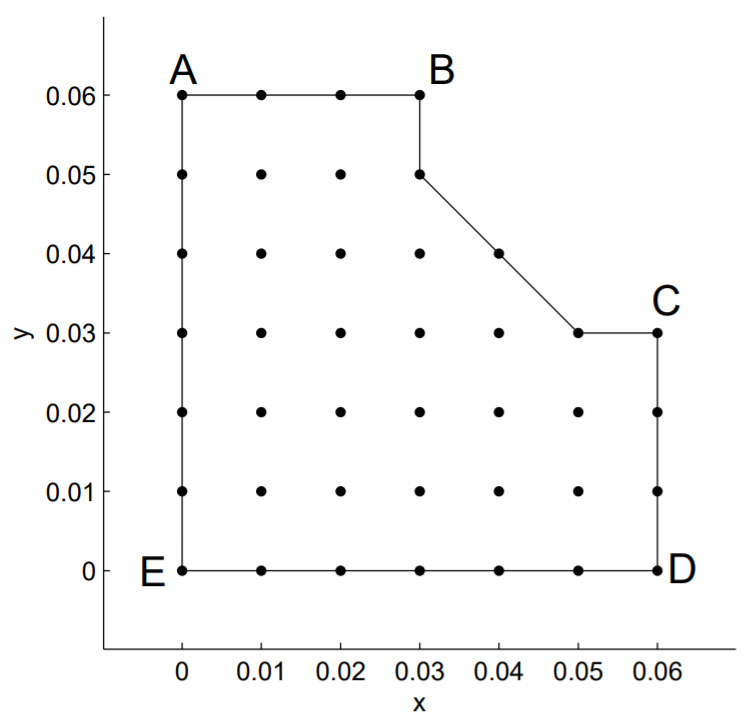
\includegraphics[width=0.9\linewidth]{images/Component.png}
	\caption{Schematic of electronic component.}
	\label{fig:componentSchematic}
\end{figure}

The component schematic is shown in Figure \ref{fig:componentSchematic}. The location of the component within the device means it's subject to different temperature condition along it's boundaries. The boundary A-B is in perfect thermal contact with another component which the temperature is known to 70\degree C. The boundary C-D is also in perfect thermal contact with another component which the temperature is known to be 40\degree C. The boundary A-E-D is thermally insulated and the boundary B-C is exposed to the air at ambient temperature.
\\\\
This type of model can be described with Laplace's equation. Letting $T(x,y)$ represent the temperature of the component at point $(x, y)$, the model is as follows	

\begin{center}
\begin{tabular}{c c}
$\frac{\partial^2 T}{\partial x^2}+\frac{\partial^2 T}{\partial y^2}=0$ & in the interior\\
$T = 70$ & on boundary A-B \\
$T = 40$ & on boundary C-D \\
$\boldsymbol{\nabla} T \cdot {\hat{\textbf{n}}} = 0$ & on boundary A-E-D\\
$k\boldsymbol{\nabla}T\cdot\hat{\textbf{n}} = h(T_{\infty} - T)$ & on boundary B-C
\end{tabular}
\end{center}
Where the thermal conductivity is $k=3Wm^{-1}C^{-1}$, and the heat transfer coefficient is $h=20 Wm^{-2}C^{-1}$. To begin with, we will assume the ambient temperature is $T_\infty = 20$.
\clearpage
\section{Method for Discretising the Problem}
If this was left as a continuous partial differential equation, we would need to analytically solve it. However, it can be much quicker to numerically solve this problem and still retain a high degree of accuracy with the final answers. In this section we will show how we converted the analytical problem to a numerical problem, how the mesh was constructed, the node ordering used, the linear system we derived from the mesh and discuss the matrix that was created from it.


\subsection{Constructing the Finite Difference Mesh}
Suppose we had a function $\phi(x,y,t)$ which gives the temperature at the point (x,y) on a 2-dimensional plane where t is the time since the start of the initial conditions. If the function has a steady-state solution, then it means at some point in time, any increase in time will not result in a change of temperature. This means that 
\begin{center}
$\frac{d\phi}{dx}|_{x_i}\approx\frac{\phi(x_i+\Delta x)-\phi(x_i)}{\Delta x}$,
\end{center}
where the change in $x$ along $\phi$ at the point $x_i$ is approximately the functions forward difference over the distance between nodes. We can then take the derivative of this again using backwards difference to get the second derivative centred around $x_i$.
\begin{center}
$\frac{d^2\phi}{dx^2}|_{x_i}\approx\frac{\phi(x_i+\Delta x)-2\phi(x_i)+\phi(x_i-\Delta x)}{(\Delta x)^2}$,
\end{center}
If we do the same for the change in $y$, we arrive at an analogous equation
\begin{center}
$\frac{d^2\phi}{dy^2}|_{y_i}\approx\frac{\phi(y_i+\Delta y)-2\phi(y_i)+\phi(y_i-\Delta y)}{(\Delta y)^2}$,
\end{center}
To numerically solve this problem, a finite difference mesh must be constructed and a matrix must be created to represent this information.
\\\\
By splitting the component up into intervals of 0.01 in both the $x$ and $y$ direction, the component can be split into a $7 \times 7$ grid. Because we know that the temperature on the upper and right hand boundaries are fixed temperatures, we can ignore them in our discretisation as nodes. They will come into effect later as the right hand side matrix. Given the previous mesh from the introduction, we can label each node u$_{i,j}$ for $i,j = 0$ to 6 where $i, j$ are given by the row and column of the node starting from the bottom left hand corner. Replacing $\phi(x,y,t)$ with $u_{i,j}(t)$ and noting that $\Delta x = \Delta y$, we arrive at the set of equations for the change in $u_{i,j}(t)$.
\begin{center}
$u'_{i,j}(t)\approx\frac{D}{\Delta x^2}\big{(}-u_{i+1,j}(t)-u_{i,j+1}(t)+4u_{i,j}(t)-u_{i-1,j}(t)-u_{i,j-1}(t)\big{)}.$
\end{center}
Note that since we are finding a state where the temperature does not change in time $(u'_{i,j}(t)=0)$, and assuming that $D\neq0$, we can rewrite this to be
\begin{center}
  $0=\big{(}-u_{i+1,j}-u_{i,j+1}+4u_{i,j}-u_{i-1,j}-u_{i,j-1}\big{)}.$
\end{center}
There are 3 different types of mesh that need to be created. These are for the A-E-D boundary, the interior of the mesh, and on the B-C boundary.
\subsubsection{Interior Nodes}
On the interior of the mesh, each node contains 4 other nodes adjacent to it, and the change in temperature at that node is given by the equation
\begin{center}
\[\frac{\partial^2 T}{\partial x^2}+\frac{\partial^2 T}{\partial y^2}=0\]
\[\frac{2T-T_W-T_E}{(0.01)^2}+\frac{2T-T_N-T_S}{(0.01)^2}=0\]
\[4T-T_W-T_E-T_N-T_S=0\]
\end{center}
\begin{center}
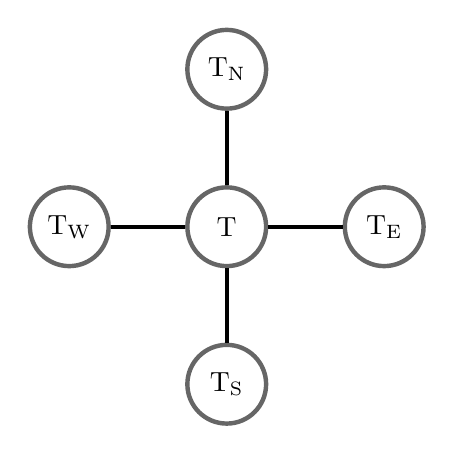
\begin{tikzpicture}[
roundnode/.style={circle, draw=black!60, ultra thick,  minimum size=10mm},
]
\node[roundnode] (center) {T};
\node[roundnode] (left) [left of=center] {T$_\text{W}$};
\node[roundnode] (right) [right of=center] {T$_\text{E}$};
\node[roundnode] (above) [above of=center] {T$_\text{N}$};
\node[roundnode] (below) [below of=center] {T$_\text{S}$};

\draw[ultra thick,-] (left.east) -- (center.west);
\draw[ultra thick,-] (above.south) -- (center.north);
\draw[ultra thick,-] (right.west) -- (center.east);
\draw[ultra thick,-] (below.north) -- (center.south);
\end{tikzpicture}
\end{center}
As an example, the node $T_{(1,1)}$ can be examined.
\begin{center}
  $4T_{(1,1)}-T_{(0,1)}-T_{(2,1)}-T_{(1,2)}-T_{(1,0)}=0$
\end{center}
\subsubsection{Boundary A-E-D Nodes}
On the boundary A-E-D, there are no nodes outside of the matrix. We can approximate them using first order forward differences (to keep the A matrix SPD). This approximation can be done using the rule $\boldsymbol{\nabla} T \cdot {\hat{\textbf{n}}} = 0$, where ${\hat{\textbf{n}}}$ is the normal unit vector at the node T and $\boldsymbol{\nabla} T$ is the directional gradient at T. The first order differences are then used to construct a finite difference equations for each node on the boundary.\\We will provide 3 examples that show all the unique cases along the boundary A-E-D, namely on the border A-E (not including A or E), the border E-D (not including E or D) and the node E.
\paragraph*{Nodes A-E}
On the A-E nodes, the normal unit vector will face directly west.
\begin{center}
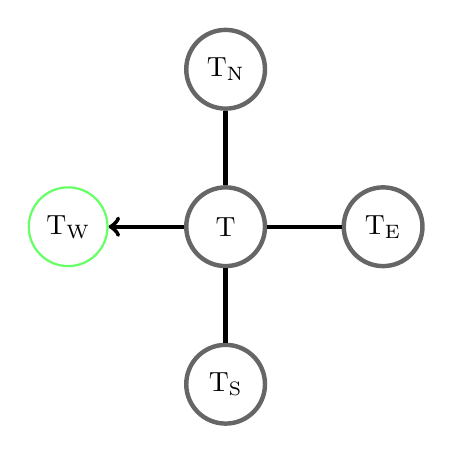
\begin{tikzpicture}[
roundnode/.style={circle, draw=black!60, ultra thick,  minimum size=10mm},
ghostnode/.style={circle, draw=green!60, thick, minimum size = 10mm},
]
\node[roundnode] (center) {T};
\node[ghostnode] (left) [left of=center] {T$_\text{W}$};
\node[roundnode] (right) [right of=center] {T$_\text{E}$};
\node[roundnode] (above) [above of=center] {T$_\text{N}$};
\node[roundnode] (below) [below of=center] {T$_\text{S}$};

\draw[ultra thick,<-] (left.east) -- (center.west);
\draw[ultra thick,-] (above.south) -- (center.north);
\draw[ultra thick,-] (right.west) -- (center.east);
\draw[ultra thick,-] (below.north) -- (center.south);
\end{tikzpicture}
\end{center}
Therefore $\hat{\textbf{n}} = (-1,0)^T$. We can construct a first order forward difference approximation for $T_W$.
\begin{center}
\[\bigg{(}\frac{\partial T_W}{\partial x},\frac{\partial T}{\partial y}\bigg{)}\cdot (-1,0)^T = 0\]
\[-\frac{\partial T_W}{\partial x} = 0\]
\[-\frac{T-T_W}{0.01} = 0\]
\[T_W = T.\]
\end{center}
This value of $T_W$ can be used in the stencil around the point T.
\begin{center}
\[\frac{\partial^2 T}{\partial x^2}+\frac{\partial^2 T}{\partial y^2}=0\]
\[\frac{2T-T_W-T_E}{(0.01)^2}+\frac{2T-T_N-T_S}{(0.01)^2}=0\]
\[2T-T_W-T_E+2T-T_N-T_S=0\]
\[4T-T-T_E-T_N-T_S=0\]
\[3T-T_E-T_N-T_S=0.\]
\end{center}

As an example, let's look at node $T_{(0, 3)}$. 
\begin{center}
  $3T_{(0,3)}-T_{(1,3)}-T_{(0,4)}-T_{(0,2)}=0$
\end{center}

\paragraph*{The Node E:}
On the node E, or (0,0) the unit normal vector will be facing south-west.
\begin{center}
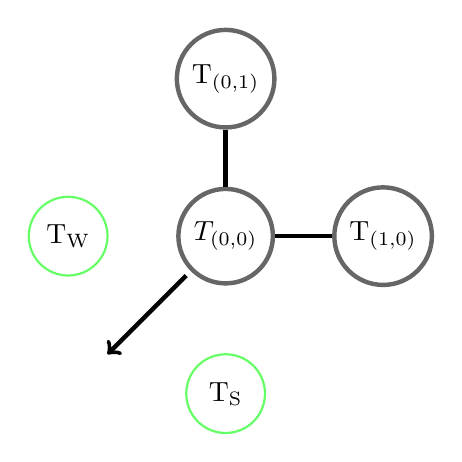
\begin{tikzpicture}[
roundnode/.style={circle, draw=black!60, ultra thick,  minimum size=10mm},
ghostnode/.style={circle, draw=green!60, thick, minimum size = 10mm},
]
\node[roundnode] (center) {$T_{(0,0)}$};
\node[ghostnode] (left) [left of=center] {T$_\text{W}$};
\node[roundnode] (right) [right of=center] {T$_{(1,0)}$};
\node[roundnode] (above) [above of=center] {T$_{(0,1)}$};
\node[ghostnode] (below) [below of=center] {T$_\text{S}$};


\draw[ultra thick,-] (above.south) -- (center.north);
\draw[ultra thick,-] (right.west) -- (center.east);
\draw[ultra thick,->] (-0.5,-0.5) -- (-1.5,-1.5);

\end{tikzpicture}
\end{center}
As a normalised vector, it will be 
\begin{center}
    $\hat{\textbf{n}} = \frac{1}{\sqrt{2}}(-1,-1)^T$.
\end{center}
We can use this in our boundary condition to create a first order difference approximation for $T_W + T_S$.
\begin{center}
  \[\bigg{(}\frac{\partial T_W}{\partial x},\frac{\partial T_S}{\partial y}\bigg{)}\cdot \frac{1}{\sqrt{2}}(-1,-1)^T = 0\]
  \[\bigg{(}\frac{\partial T_W}{\partial x},\frac{\partial T_S}{\partial y}\bigg{)}\cdot (-1,-1)^T = 0\]
  \[-\bigg{(}\frac{\partial T_W}{\partial x}-\frac{\partial T_S}{\partial y}\bigg{)} = 0\]
  \[\frac{T-T_W}{0.01}+\frac{T-T_S}{0.01} = 0\]
  \[T_W+T_S=2T.\]
\end{center}
Substituting this into our stencil, we can see that 
\begin{center}
\[4T_{(0,0)}-T_{(0,1)}-T_{(1,0)}-T_{W}-T{S}=0\]
\[4T_{(0,0)}-T_{(0,1)}-T_{(1,0)}-2T_{(0,0)}=0\]
\[2T_{(0,0)}-T_{(0,1)}-T_{(1,0)}=0.\]
\end{center}

\paragraph*{Nodes E-D:} On the nodes E-D, the normal unit vector will face directly south. 
\begin{center}
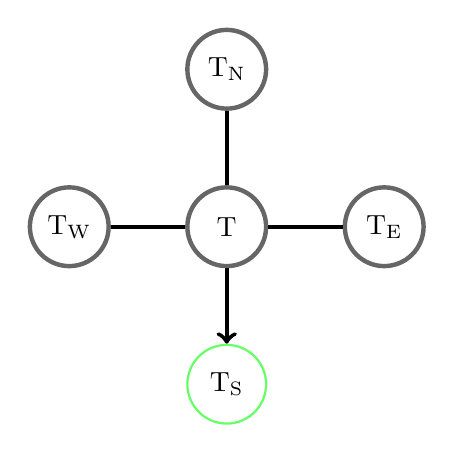
\begin{tikzpicture}[
roundnode/.style={circle, draw=black!60, ultra thick,  minimum size=10mm},
ghostnode/.style={circle, draw=green!60, thick, minimum size = 10mm},
]
\node[roundnode] (center) {T};
\node[roundnode] (left) [left of=center] {T$_\text{W}$};
\node[roundnode] (right) [right of=center] {T$_\text{E}$};
\node[roundnode] (above) [above of=center] {T$_\text{N}$};
\node[ghostnode] (below) [below of=center] {T$_\text{S}$};

\draw[ultra thick,-] (left.east) -- (center.west);
\draw[ultra thick,-] (above.south) -- (center.north);
\draw[ultra thick,-] (right.west) -- (center.east);
\draw[ultra thick,<-] (below.north) -- (center.south);
\end{tikzpicture}
\end{center}
This can be written as 
\begin{center}
  $\hat{\textbf{n}}=(0,-1)^T$.
\end{center}
Using the same boundary rule for the edge A-E-D (which contains the edge E-D) we can find a first order forward difference for $T_S$.
\begin{center}
\[\bigg{(}\frac{\partial T_S}{\partial x},\frac{\partial T}{\partial y}\bigg{)}\cdot (0,-1)^T = 0\]
\[-\frac{\partial T_S}{\partial y}=0\]
\[-\frac{T-T_S}{0.01}=0\]
\[T_S=T\]
\end{center} 
Using this in our finite difference equation, we get the following equation for a node along the boundary E-D.
\begin{center}
  \[4T-T_S-T_N-T_W-T_E=0\]
  \[4T-T-T_N-T_W-T_E=0\]
  \[3T-T_N-T_W-T_E=0.\]
\end{center}
As an example, let us look at node $T_{(3,0)}$.
\begin{center}
  $3T_{(3,0)}-T_{(3,1)}-T_{(2,0)}-T_{(4,0)}=0$.
\end{center}
Each other node along the boundary will be similar to this node.
\subsubsection{Boundary B-C}
There are three nodes that we care about on the boundary B-C. The boundary condition along these nodes are
\[k\boldsymbol{\nabla}T\cdot\hat{\textbf{n}} = h(T_{\infty} - T)\]
where $k=3\text{Wm}^{-1}\text{C}^{-1}, h=20\text{Wm}^{-2}\text{C}^{-1}, T_\infty=20$.


\begin{center}
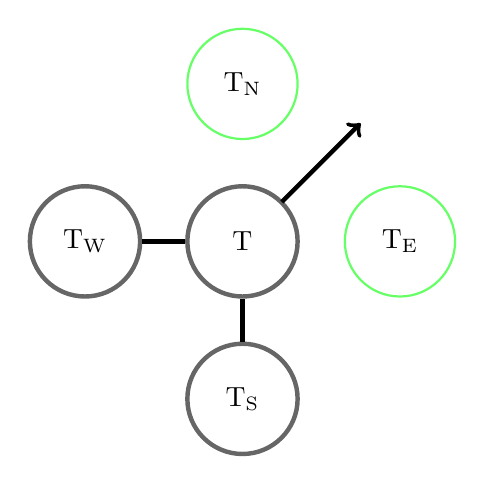
\begin{tikzpicture}[
roundnode/.style={circle, draw=black!60, ultra thick,  minimum size=14mm},
ghostnode/.style={circle, draw=green!60, thick, minimum size = 14mm},
]
\node[roundnode] (center) {T};
\node[roundnode] (left) [left of=center] {T$_\text{W}$};
\node[ghostnode] (right) [right of=center] {T$_\text{E}$};
\node[ghostnode] (above) [above of=center] {T$_\text{N}$};
\node[roundnode] (below) [below of=center] {T$_\text{S}$};

\draw[ultra thick,-] (left.east) -- (center.west);
\draw[ultra thick,->] (0.5,0.5) -- (1.5,1.5);
\draw[ultra thick,-] (below.north) -- (center.south);
\end{tikzpicture}
\end{center}
The unit normal on each node will be facing directly northeast as the boundary is diagonal. Therefore
\[\hat{\textbf{n}} = \frac{1}{\sqrt{2}}(1,1)^T.\]
Using this in our boundary condition (along with leaving the ambient temperature as a variable) yields
\[3\bigg{(}\frac{\partial T}{\partial x},\frac{\partial T}{\partial y}\bigg{)}\cdot\frac{1}{\sqrt{2}}\big{(}1,1\big{)}^T=20\big{(}T_\infty-T\big{)}\]
Using first order forward differences for $\frac{\partial T}{\partial x}$ and $\frac{\partial T}{\partial y}$ and rearranging to solve for $\text{T}_\text{N}+\text{T}_\text{E}$
\[\frac{3}{\sqrt{2}}\bigg(\frac{T_E-T}{0.01}+\frac{T_N-T}{0.01}\bigg)=20T_\infty-20T\]
\[T_E+T_N-2T=\frac{\sqrt{2}}{3}\big(0.2T_\infty-0.2T\big)\]
\[T_E+T_N=\frac{0.2T_\infty\sqrt{2}}{3}+\frac{6-0.2\sqrt{2}}{3}T.\]
For two of the nodes along the B-C boundary, either $T_E$ or $T_N$ will be constant. 
 
\subsection{Node Ordering}
One last thing we must do is construct a mapping from the 2D array of nodes to a 1D array of nodes. This is useful when creating the vectors $x$ and $b$ in the linear equation $Ax=b$.
\\\\
Because we have a $6 \times 6$ array (ignoring the missing or null nodes in the top right corner) we can transform this into a 1D array with 36 values. We can use the following assumptions to construct the map \begin{itemize}
\item Our index is $(i,j)$ with $i$ being the horizontal coordinate and $j$ being the vertical coordinate 
\item (0,0) is the bottom left node 
\item ($i+1$, $j$) is to the right of ($i$,$j$) and ($i$,$j+1$) is above ($i$, $j$)
\end{itemize}
From this we can deduce that every time we move across the 2D array, we are moving 1 unit across in the 1D array, and every time we move up in the 2D array, we are moving 6 across in the 1D array. Therefore,
\begin{center}
$(i,j) \to i+6j$.
\end{center}
For example, the equation
\[2T_{(0,0)}-T_{(1,0)}-T_{(0,1)}=0\]
will transform into
\[2T_0-T_1-T_6=0.\]
\subsection{Matrix Construction}
Using our node ordering, we can write out all the equations in a certain ordering (See Appendix A1). This can then be rewritten as a linear system, $Ax=b$, where A is the coefficient matrix of the equations, x is the unknown temperature values and b is the right hand side values of the equations (See Appendix A2). \\\\Using our node ordering, we can write out all the equations in a certain ordering (See Appendix A). This can then be rewritten as a linear system, Ax=b, where A is the coefficient matrix of the equations, x is the unknown temperature values and b is the right hand side values of the equations (See Appendix A2). \\\\Using the spy() command on A, we can see that it has a banded structure, noting that it has a total bandwidth of 13.\\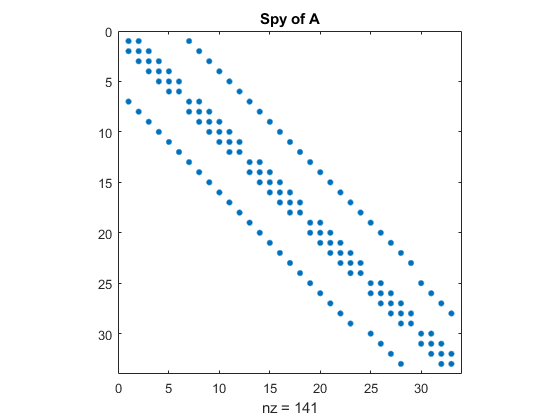
\includegraphics{images/spyA.png}
\subsection{Checking SPD}
The matrix A is both symmetric and positive definite. This can be verified with Matlab.\\If A is symmetric, then for all (i,j)$\in$ dim(A), A(i,j) = A(j,i). To check that it is symmetric, we can use the spy() command on A minus A transpose.
The matrix A is both symmetric and positive definite. This can be verified with matlab.\\If A is symmetric, then for all (i, j)$\in$ dim(A), A(i, j) = A(j, i). To check that it is symmetric, we can use the spy() command on A minus A transpose.
\begin{minted}{matlab}
	spy(A-A')
\end{minted}
The spy command produces a plot graph with plots in coordinates where the value of the matrix (at the same coordinate) is not zero. Since the figure produced by the spy command has no plots, every value in the matrix A-A' is zero, which implies that A is symmetric.\\\\To show that A is positive definite, it is enough to show that the eigenvalues are all positive. This can be done simply with the eig() command.
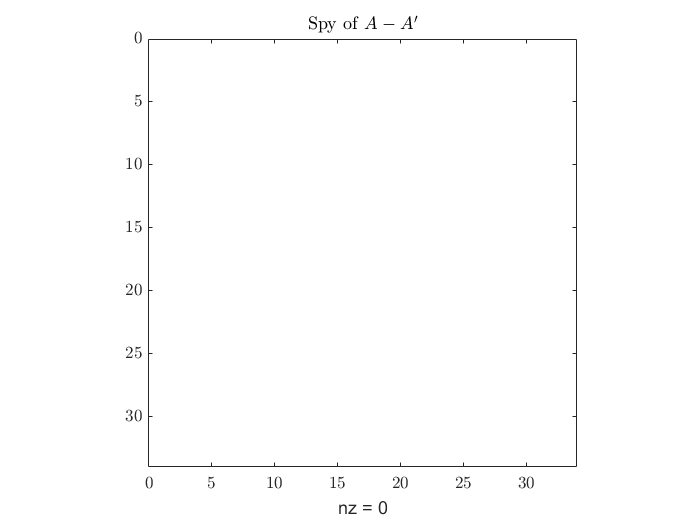
\includegraphics{images/spySymmetric.png}
The spy command produces a plot graph with plots in coordinates where the value of the matrix (at the same coordinate) is not zero. Since the figure produced by the spy command has no plots, every value in the matrix A-A' is zero, which implies that A is symmetric.\\\\To show that A is positive definite, it is enough to show that the eigenvalues are all postive. This can be done simply with the eig() command.
\begin{minted}{matlab}
	eig(A)
\end{minted}
The results of this are in Appendix A3. Because they are all positive, A is positive definite. 
The results of this are in Appendix A4. Because they are all positive, A is postive definite. 
\section{Storage and Solutions}
In this section, iterative methods and direct methods are used to solve for $x$, such that:
\\
\begin{center}
$Ax=b$.
\\
\end{center}

\subsection{Full Storage}

\subsection{Packed Storage}

\subsection{Band Storage}
A banded system is a matrix where all non-zero elements are within a certain distance of the main diagonal (which depends on the matrix). The matrix looked at previously is a banded system, however, it is not ordered in an efficient manner, as the bandwidth is unnecessarily increased due to the number of 0-diagonals between the inner tridiagonal and the outer diagonals. Using a technique called RCM 
A banded system is a matrix where all non-zero elements are within a certain distance of the main diagonal (which depends on the matrix). The matrix looked at previously is a banded system, however, it is not ordered in an efficent manner, as the bandwidth is unnecessarily increased due to the number of 0-diagonals between the inner tridiagonal and the outer diagonals. Using a technique called RCM ordering, the empty space between the outer and inner diagonals can be greatly reduced. To use this in Matlab, the following code is used
\begin{minted}{matlab}
%RCM Storage
load full_storage
%Create a new matrix to work with
A_RCM = A;
%create ordering vector
p= symrcm(A_RCM);
%order the A matrix and b vector according the RCM storage
A_RCM = A_RCM(p,p);
b_rcm = b(p);
reorder = reorder_vector(p);
\end{minted}
The b vector is also reordered using the same reordering vector to keep the equation $Ax=b$ the same. A reorder vector is created from p to reverse the rcm ordering for when the system of equations is solved for the steady state temperatures. The code for the reorder\_vector() function is
\begin{minted}{matlab}
function p = reorder_vector(b)
%Takes a reordering vector and outputs the reverse reordering vector
[~,n] = size(b);
p = zeros(n,1);
for i = 1:n
	p(b(i)) = i;
end
end
\end{minted}
The reordered A matrix using RCM ordering will look like\\
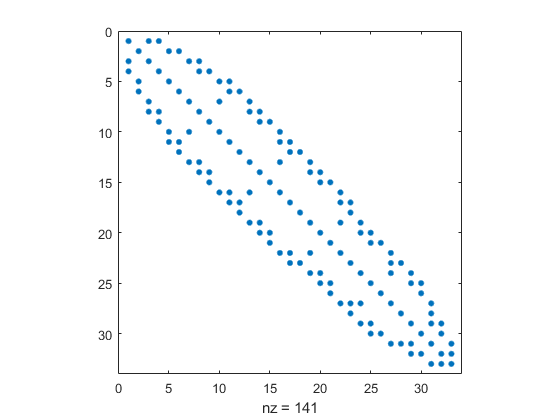
\includegraphics{images/ARCM.png}
The bandwidth of this matrix is also 13. However, more elements are closer to the main diagonal.
\\\\The next step is to convert the RCM ordering to a banded storage matrix, denoted $B$. Because $A$ is symmetric, we can get away with only storing the upper or lower part of the matrix. The dimensions of this matrix are $\mathbb{R}^{n\times p}$, where n is the row or column count of $A$, and p is the upper bandwidth of $A$. To change the storage, we must create a new mapping from the elements of the upper portion of $A$ to $B$.
\begin{align*}
A(i,j)\to B(i,j-i+1), \text{ where } i,j < \text{dim}(A).
\end{align*}
The Matlab code to implement this is
\begin{minted}{matlab}
function B = band(A)
[n,~] = size(A);
m = bandwidth(A)+1;
B = zeros(n,m);
for i = 1:n
	for j = 1:m
		if (i + j < n+2)
			B(i,j) = A(i,j+i-1);
		end
	end
end
end
\end{minted}
The (transposed) resulting matrix will look like \\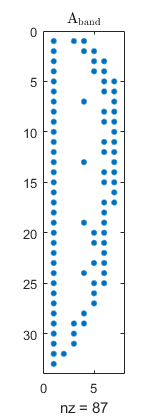
\includegraphics{images/band.png}
To perform Cholesky factorisation on this matrix, and keeping the factorised matrix in the same dimension, the regular Cholesky factorisation method can be retooled using the previously mentioned mapping for band storage. The new Band Cholesky factorisation method will be
\begin{minted}{matlab}
function [A, flops] = cholesky_band(A, current_flops)
[n,width] = size(A);
for j = 1:n
	for i = 1:j-1
		for k = 1:i-1
			if((j-i+1) < width+1 && (i-k+1) < width+1 && (j-k+1) < width+1)
				A(i,j-i+1) = A(i,j-i+1) - A(k,i-k+1) * A(k,j-k+1);
			end
		end
		if(j-i+1<(width+1))
			A(i,j-i+1) = A(i,j-i+1) / A(i,1);
			A(j,1) = A(j,1) - A(i,j-i+1)^2;
		end
	end
	A(j,1) = sqrt(A(j,1));
end	
\end{minted}
The new algorithm must now check that the index $j-i+1$ is within the width of the matrix, as the column is less than the row count, and trying to access $A(i,j-i+1)$ would result in an error if $j-i+1$ was greater than the number of columns. In the original matrix, these values would have just been 0, and no change would happen.\\\\Performing the Banded Cholesky algorithm on the banded matrix yields (as a transposed figure) \\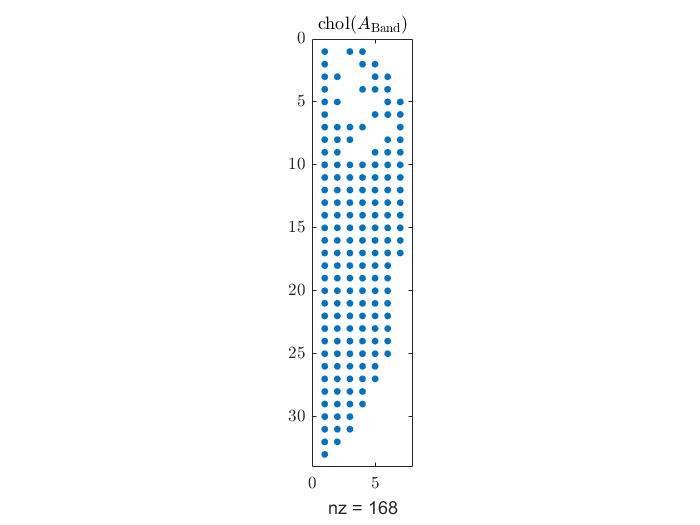
\includegraphics{images/cholband.png}
To use this factorised matrix, a new forward and backward method must be constructed. Luckily, the previous mapping can still be used. Care must be taken when working in a non-square matrix in both forward and backward substitution as well.
\subsection{Sparse Storage}

\subsection{Compressed Sparse Row Format Storage}
\textbf{Compressed sparse row format} (CSR), stores all the non-zero elements that are in a given matrix and it's respected row and column indices of these non-zero elements. CSR consists of three arrays: \textbf{rb} which stores the index of where each new row begins in both \textbf{c} and \textbf{v}; \textbf{c} which consists of the column indices; and \textbf{v} which contains the value of these elements. $\textbf{rb}$ ends with $nz + 1$, where $nz$ is the total number of non-zero elements in $A$.
\\\\
CSR storage was used to factorise $A$. Jacobi, Gauss-Seidel, Successive Over-relaxation (SOR), Conjugate Gradient Methods were used to solve for $x$.
\\\\
To factorise $A$ using CSR storage, the matrix had to first be sorted into three vectors $\textbf{r}$, $\textbf{c}$, and $\textbf{v}$, where $\textbf{r}$ was the row indices. T using Matlab's built in function: 
\begin{minted}{matlab} 
[r, c, v] = find(A) 
\end{minted}
This function returns $\textbf{r}$, $\textbf{c}$, and $\textbf{v}$ where the column indices are in ascending order. Therefore, $\textbf{r}$ must be ordered so the row indices are in ascending order and $\textbf{c}$, and $\textbf{v}$ needed to be reordered to correctly represent $A$. Then, $\textbf{r}$ must to be converted to $\textbf{rb}$.

\subsubsection{The Jacobi Method}
The first iterative method that is used to solve CSR is the Jacobi method. 

\subsubsection{The Gauss-Seidel Method}

\subsubsection{The Successive Over-relaxation Method}

\subsubsection{The Conjugate Gradient Method}

\subsection{Visualisation}

\section{Efficiency Comparison}
The following section investigates which numerical method or methods provide the greatest efficiency in solving problems similar to the electronic component.

\subsection{Bandwidth and level of fill-in for Each Different Node Ordering}


\subsection{Memory (for Direct Methods)}
\begin{center}
\begin{tabular}{c c c c c}
Name & Size & Bytes & Class & Attributes \\
\hline
$A$ & $33 \times 33$ & $8712$ & double & \\
$A$ Banded Storage & $33 \times 7$ & $1848$ & double & \\
$A$ Packed Storage & $1 \times 561$ & $4488$ & double & \\
$A$ Sparse Storage & $33 \times 33$ & $2528$ & double & sparse \\
$b$ & $33 \times 1$ & $264$ & double & \\
\end{tabular}
\end{center}

\begin{figure}[H]
	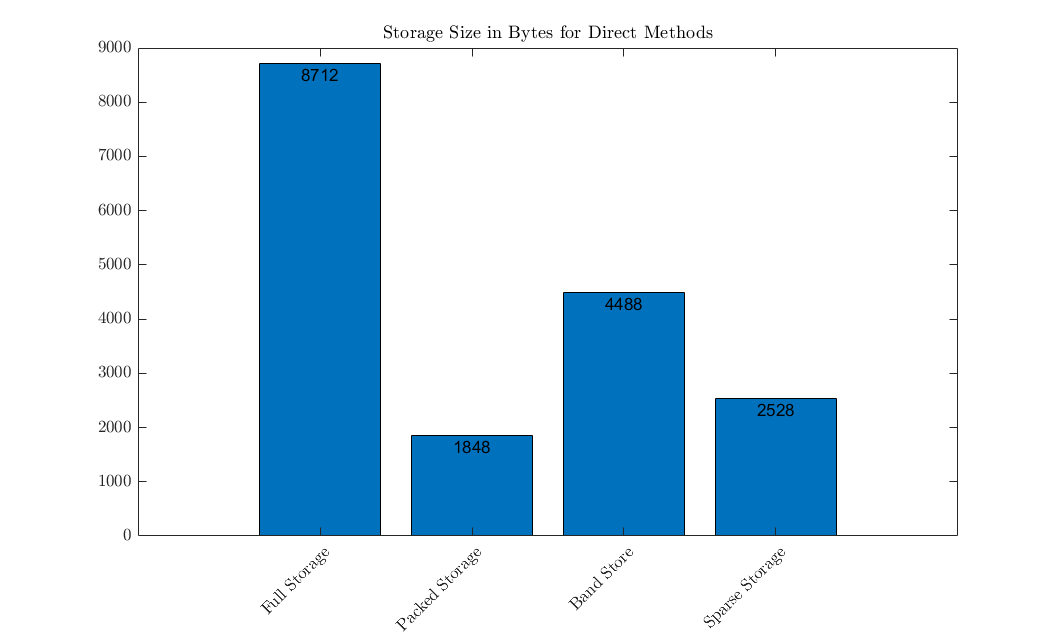
\includegraphics[width=\linewidth]{images/MemoryGraph.png}
	\caption{Memory of each of the A and b which are stored for each Direct Method.}
	\label{fig:memory}
\end{figure}

\subsection{Iterations (for Iterative Methods)}
\begin{figure}[H]
	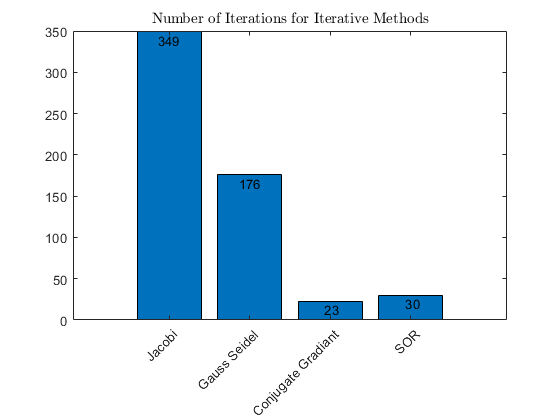
\includegraphics[width=\linewidth]{images/IterationsGraph.png}
	\caption{Number of Iterations for each Iterative Method}
	\label{fig:iterations}
\end{figure}


\subsection{Runtime (Direct and Iterative)}
\begin{figure}[H]
	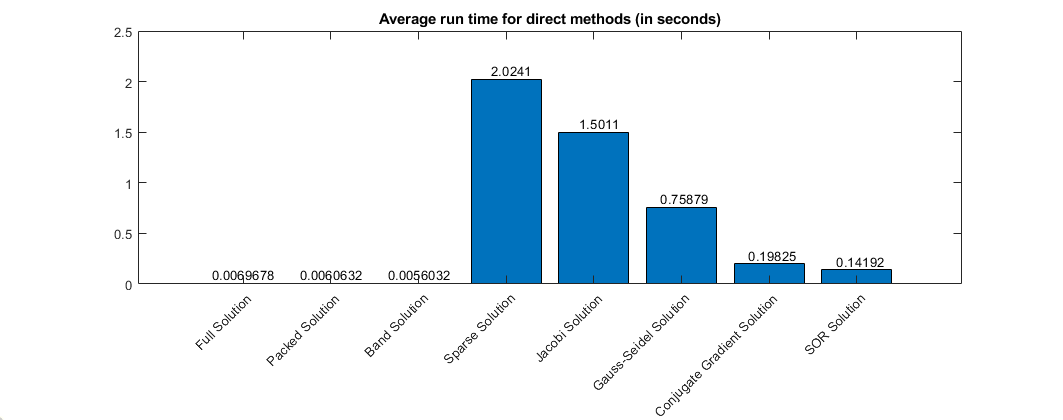
\includegraphics[width=\linewidth]{images/RuntimeGraph.png}
	\caption{Runtime for solving each of the Direct and Iterative Methods.}
	\label{fig:runtime}
\end{figure}

\subsection{Floating Point Operations (Direct and Iterative)}
\begin{figure}[H]
	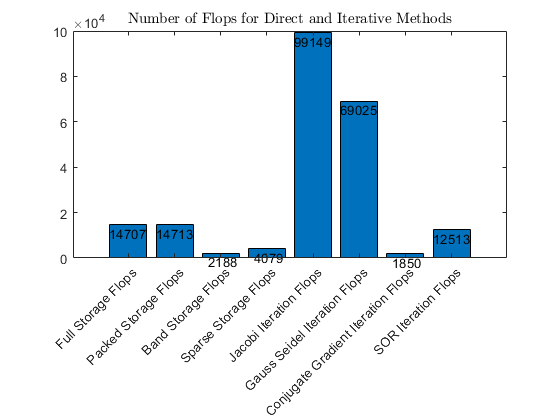
\includegraphics[width=\linewidth]{images/FlopsGraph.png}
	\caption{Flops for each Direct and Iterative Methods.}
	\label{fig:flops}
\end{figure}

\begin{figure}[H]
	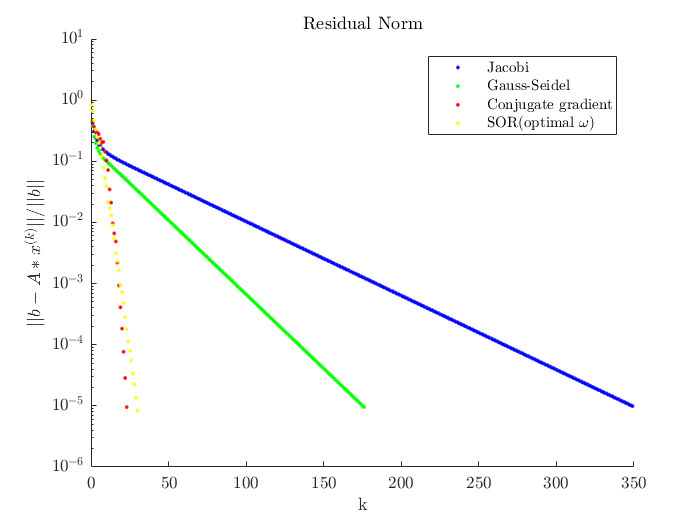
\includegraphics[width=\linewidth]{images/ResidualNormGraph.png}
	\caption{Residual Norm for each Iterative Methods}
	\label{fig:res}
\end{figure}

\subsection{Tolerance Required for Iterative Methods)}
The following discusses the tolerance that is required for the iterative methods to produce a solution that is visually indistinguishable from that produced by the direct method.
\\\\
\subsection{Effect of $\omega$ on the Rate of Convergence of the SOR Method}
The effect of $\omega$ on the rate of convergence of the SOR methods investigated. The tolerance, $10^{-5}$ was selected.
\\\\
For matrices that arise from finite difference discretisations of Laplace's equation, the value of $\omega$ that minimises the spectral radius $\rho(T_{SOR})$ is 
\begin{center}
$\omega_{opt} = \frac{2}{1+\sqrt{1-\rho(T_{J})^{2}}}$.
\end{center}
The Figure \ref{fig:omega1} compares the value of $\omega$ against $\rho(T_{SOR})$ to visually see what $\omega$ value has the least $\rho(T_{SOR})$. The theoretical optimal value of $\omega$ is $\omega_{opt}$.

\begin{figure}[H]
	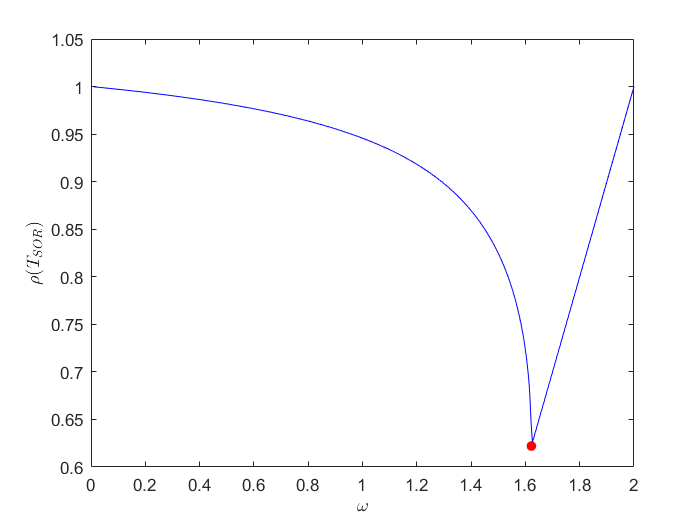
\includegraphics[width=\linewidth]{images/omegaGraph1.png}
	\caption{Omega.}
	\label{fig:omega1}
\end{figure}

The effect of $\omega$ was explored on the number of iterations taken to converge. In Figure \ref{fig:omega2} it can be seen that the $\omega$ that had the least iterations to converge was $\omega_{opt}$. Thus, the $\omega$ that will result with the least amount of iterations is approximately $1.605$.

\begin{figure}[H]
	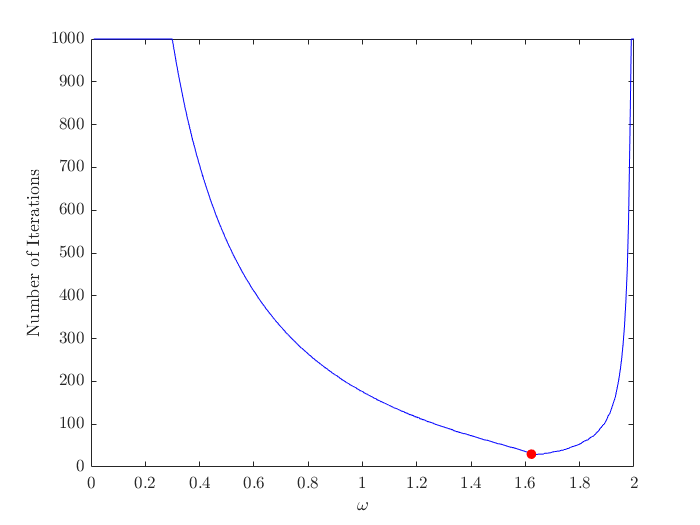
\includegraphics[width=\linewidth]{images/omegaGraph2.png}
	\caption{Number of Iterations against different values of $\omega$.}
	\label{fig:omega2}
\end{figure}

%
%\subsection{Method}
%
%\subsubsection{Procedures}
%
%\subsubsection{Sample Size}
%
%\subsubsection{Selection Criteria}
%
%\subsection{Discussion and analysis of data}
%
%\subsubsection{Issue 1}
%
%\subsubsection{Issue 2}
%
%\subsubsection{Issue 3}
%
%\subsubsection{Reliability and accuracy of data}
%
%\section{Conclusions}
%
%\section{Recommendations}
%
%\subsection{Recommendation 1}
%
%\subsection{Recommendation 2}
%
%\section{References}
%
\section{Appendices}
\subsection*{Appendix A}
\begin{align*}
2\text{T}_0-\text{T}_1-\text{T}_6              & =0\\
3\text{T}_1-\text{T}_0-\text{T}_2-\text{T}_7          & =0\\
3\text{T}_2-\text{T}_1-\text{T}_3-\text{T}_8          & =0\\
3\text{T}_3-\text{T}_2-\text{T}_4-\text{T}_9          & =0\\
3\text{T}_4-\text{T}_3-\text{T}_5-\text{T}_{10}       & =0\\
3\text{T}_5-\text{T}_4-\text{T}_{11}           & =40\\
3\text{T}_6-\text{T}_0-\text{T}_7-\text{T}_{12}       & =0\\
4\text{T}_7-\text{T}_8-\text{T}_1-\text{T}_6-\text{T}_{13}   & =0\\
4\text{T}_8-\text{T}_7-\text{T}_2-\text{T}_9-\text{T}_{14}   & =0\\
4\text{T}_9-\text{T}_8-\text{T}_3-\text{T}_{10}-\text{T}_{15}& =0\\
4\text{T}_{10}-\text{T}_9-\text{T}_4-\text{T}_{11}-\text{T}_{16} & =0\\
4\text{T}_{11}-\text{T}_{10}-\text{T}_5-\text{T}_{17} & =40\\
3\text{T}_{12}-\text{T}_6-\text{T}_{16}-\text{T}_{13} & =0\\
4\text{T}_{13}-\text{T}_{12}-\text{T}_{14}-\text{T}_{7}-\text{T}_{19} & =0\\
4\text{T}_{14}-\text{T}_{13}-\text{T}_{15}-\text{T}_{8}-\text{T}_{20} & =0\\
4\text{T}_{15}-\text{T}_{14}-\text{T}_{16}-\text{T}_{9}-\text{T}_{21} & =0\\
4\text{T}_{16}-\text{T}_{15}-\text{T}_{17}-\text{T}_{10}-\text{T}_{22}& =0\\
4\text{T}_{17}-\text{T}_{16}-\text{T}_{11}-\text{T}_{23} & =40\\
3\text{T}_{18}-\text{T}_{12}-\text{T}_{24}-\text{T}_{19} & =0\\
4\text{T}_{19}-\text{T}_{18}-\text{T}_{20}-\text{T}_{13}-\text{T}_{25} & =0\\
4\text{T}_{20}-\text{T}_{19}-\text{T}_{21}-\text{T}_{14}-\text{T}_{26} & =0\\
4\text{T}_{21}-\text{T}_{20}-\text{T}_{22}-\text{T}_{15}-\text{T}_{27} & =0\\
4\text{T}_{22}-\text{T}_{21}-\text{T}_{23}-\text{T}_{16}-\text{T}_{28} & =0\\
\frac{9.2}{3}\text{T}_{23}-\text{T}_{22}-\text{T}_{17} & =40+\frac{4}{3}\\
3\text{T}_{24}-\text{T}_{18}-\text{T}{30}-\text{T}_{25} &=0\\
4\text{T}_{25}-\text{T}_{24}-\text{T}_{26}-\text{T}_{19}-\text{T}_{31} & =0\\
4\text{T}_{26}-\text{T}_{25}-\text{T}_{27}-\text{T}_{20}-\text{T}_{32} & =0\\
4\text{T}_{27}-\text{T}_{26}-\text{T}_{28}-\text{T}_{21}-\text{T}_{33} & =0\\
\bigg(2+\frac{0.2\sqrt{2}}{3}\bigg)\text{T}_{28}-\text{T}_{27}-\text{T}_{22} & =\frac{4\sqrt{2}}{3}\\
\text{T}_{29} \text{ is null}\\
3\text{T}_{30}-\text{T}_{24}-\text{T}_{31} &=70\\
4\text{T}_{31}-\text{T}_{30}-\text{T}_{32}-\text{T}_{25} &=70\\
4\text{T}_{32}-\text{T}_{31}-\text{T}_{33}-\text{T}_{26} &=70\\
\frac{9.2}{3}\text{T}_{33}-\text{T}_{32}-\text{T}_{27} & =70+\frac{4}{3}\\
\text{T}_{34} \text{ is null}\\
\text{T}_{35} \text{ is null}
\end{align*}
\subsection*{Appendix B}
\begin{figure}
	\centering
	\begin{subfigure}[b]{0.4\textwidth}
		\centering
		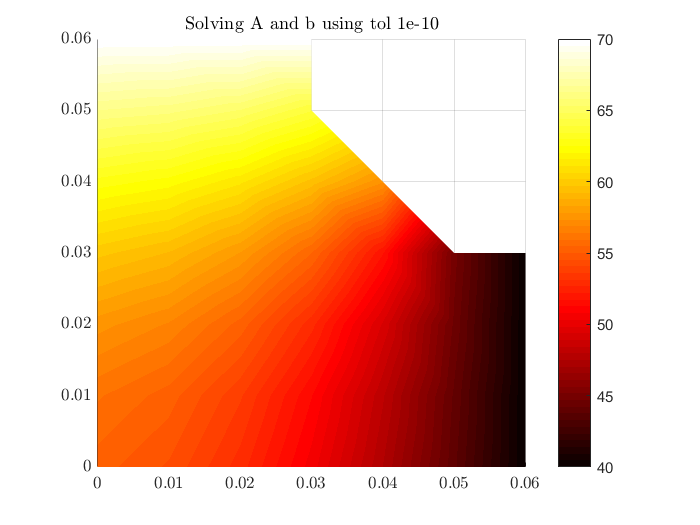
\includegraphics[width=\textwidth]{images/Comparisontole-10.png}
		\caption{Tolerance of $10^{-10}$.}
		\label{fig:tole-10}
	\end{subfigure}
	\hfill
	\begin{subfigure}[b]{0.4\textwidth}
		\centering
		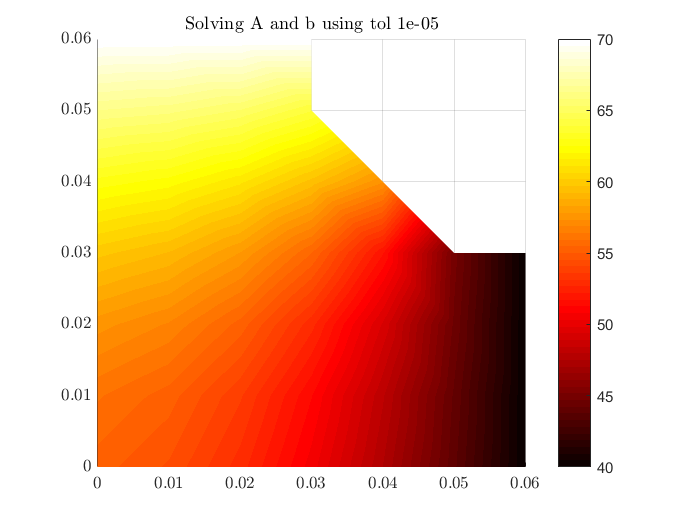
\includegraphics[width=\linewidth]{images/Comparisontole-05.png}
		\caption{Tolerance of $10^{-5}$.}
		\label{fig:tole-05}
	\end{subfigure}
	\hfill
	\begin{subfigure}[b]{0.4\textwidth}
		\centering
		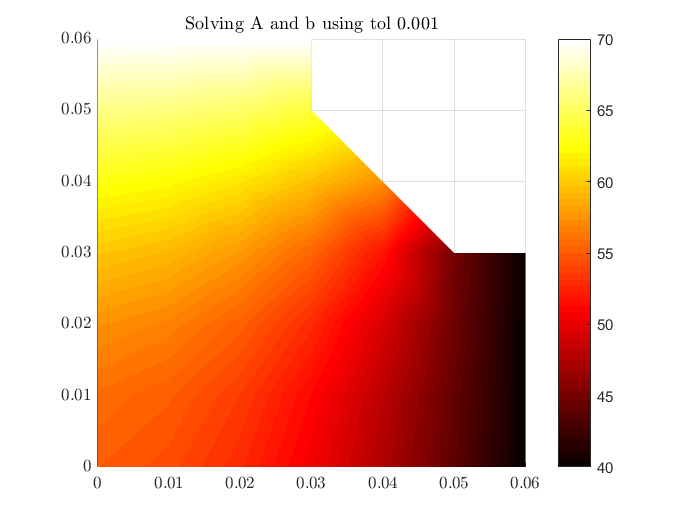
\includegraphics[width=\linewidth]{images/Comparisontol0-001.png}
		\caption{Tolerance of $10^{-3}$.}
		\label{fig:tol0.001}
	\end{subfigure}
	\hfill
	\begin{subfigure}[b]{0.4\textwidth}
		\centering
		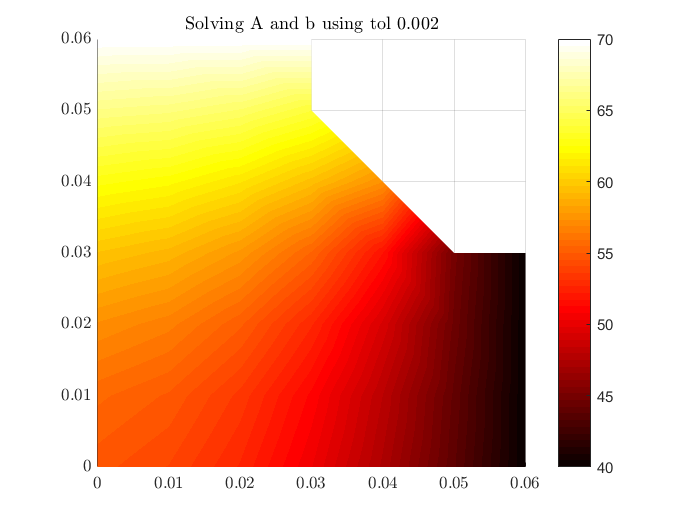
\includegraphics[width=\linewidth]{images/Comparisontol0-002.png}
		\caption{Tolerance of $2 \times 10^{-3}$.}
		\label{fig:tol0.002}
	\end{subfigure}
	\hfill
	\begin{subfigure}[b]{0.4\textwidth}
		\centering
		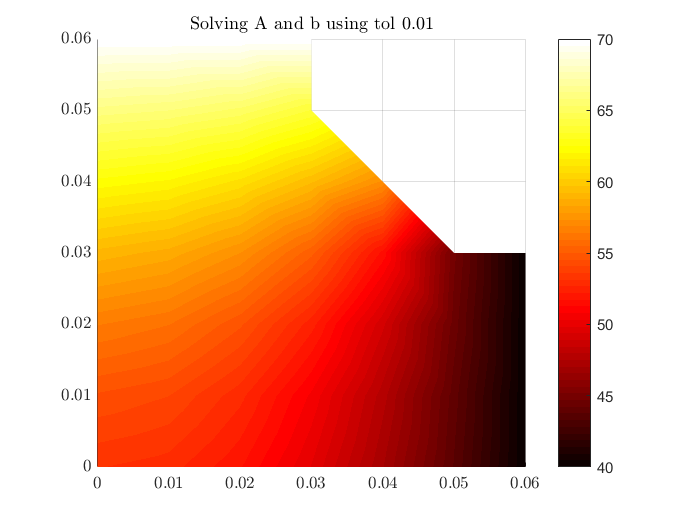
\includegraphics[width=\linewidth]{images/Comparisontol0-01.png}
		\caption{Tolerance of $10^{-2}$.}
		\label{fig:tol0.01}
	\end{subfigure}
	\hfill
	\begin{subfigure}[b]{0.4\textwidth}
		\centering
		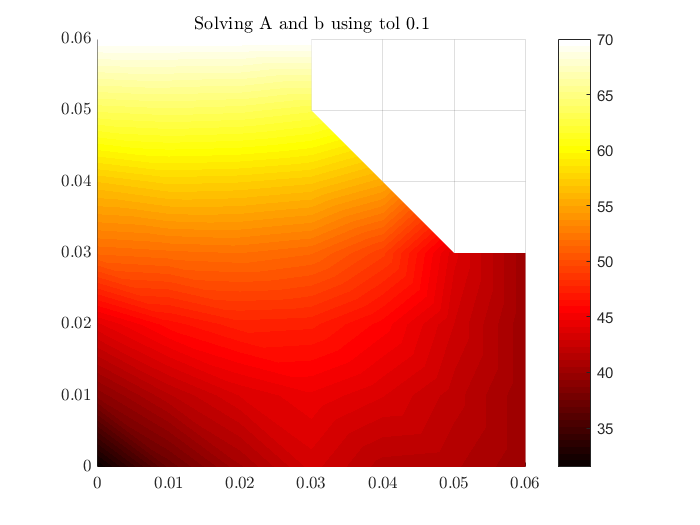
\includegraphics[width=\linewidth]{images/Comparisontol0-1.png}
		\caption{Tolerance of $10^{-1}$.}
		\label{fig:tol0.1}
	\end{subfigure}
	\hfill
	\begin{subfigure}[b]{0.4\textwidth}
		\centering
		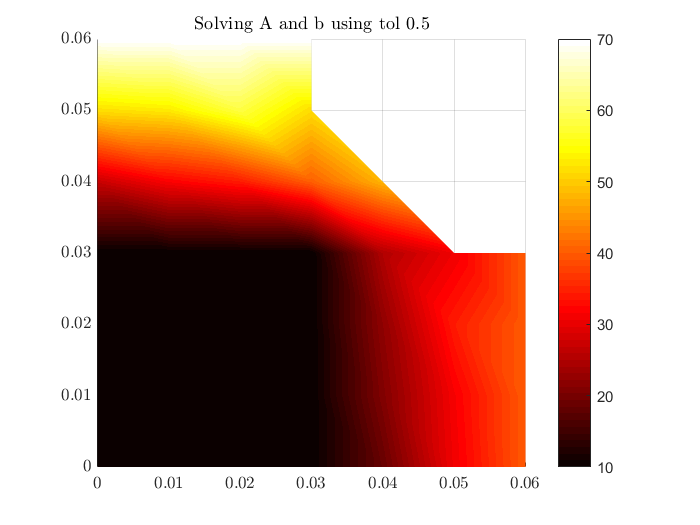
\includegraphics[width=\linewidth]{images/Comparisontol0-5.png}
		\caption{Tolerance of $0.5$.}
		\label{fig:tol0.5}
	\end{subfigure}
	\hfill
	\begin{subfigure}[b]{0.4\textwidth}
		\centering
		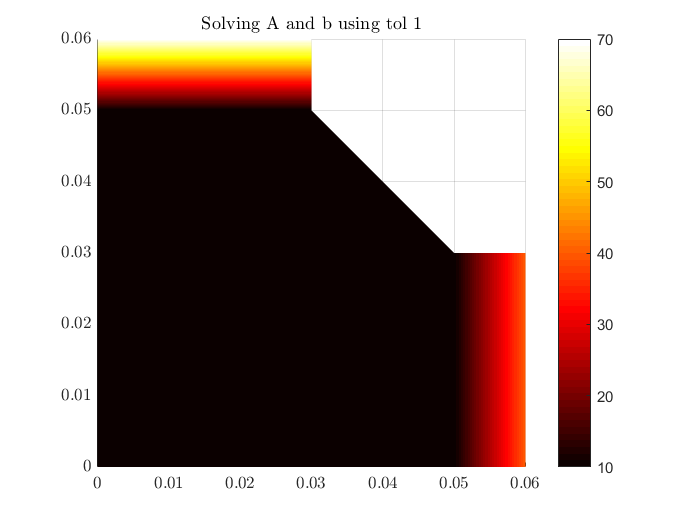
\includegraphics[width=\linewidth]{images/Comparisontol1.png}
		\caption{Tolerance of $1$.}
		\label{fig:tol1}
	\end{subfigure}
	\caption{Varying tolerances for solving $x$ using the SOR Method.}
    \label{fig:tolerance}
\end{figure}
 
\end{document}
